Ebenso wie beim UEQ, sollten die Probanden sich auch beim SUS-Fragebogen nur 
auf den Einrichtungsprozess selbst beziehen und auf die Handhabung der Blue 
TOTP App sowie der Blue TOTP Extension.
\\\\
Die SUS-Bewertungen sind in Abb. \ref{fig: studie setup sus boxplot} zu sehen. 
\begin{figure}
    \centering
    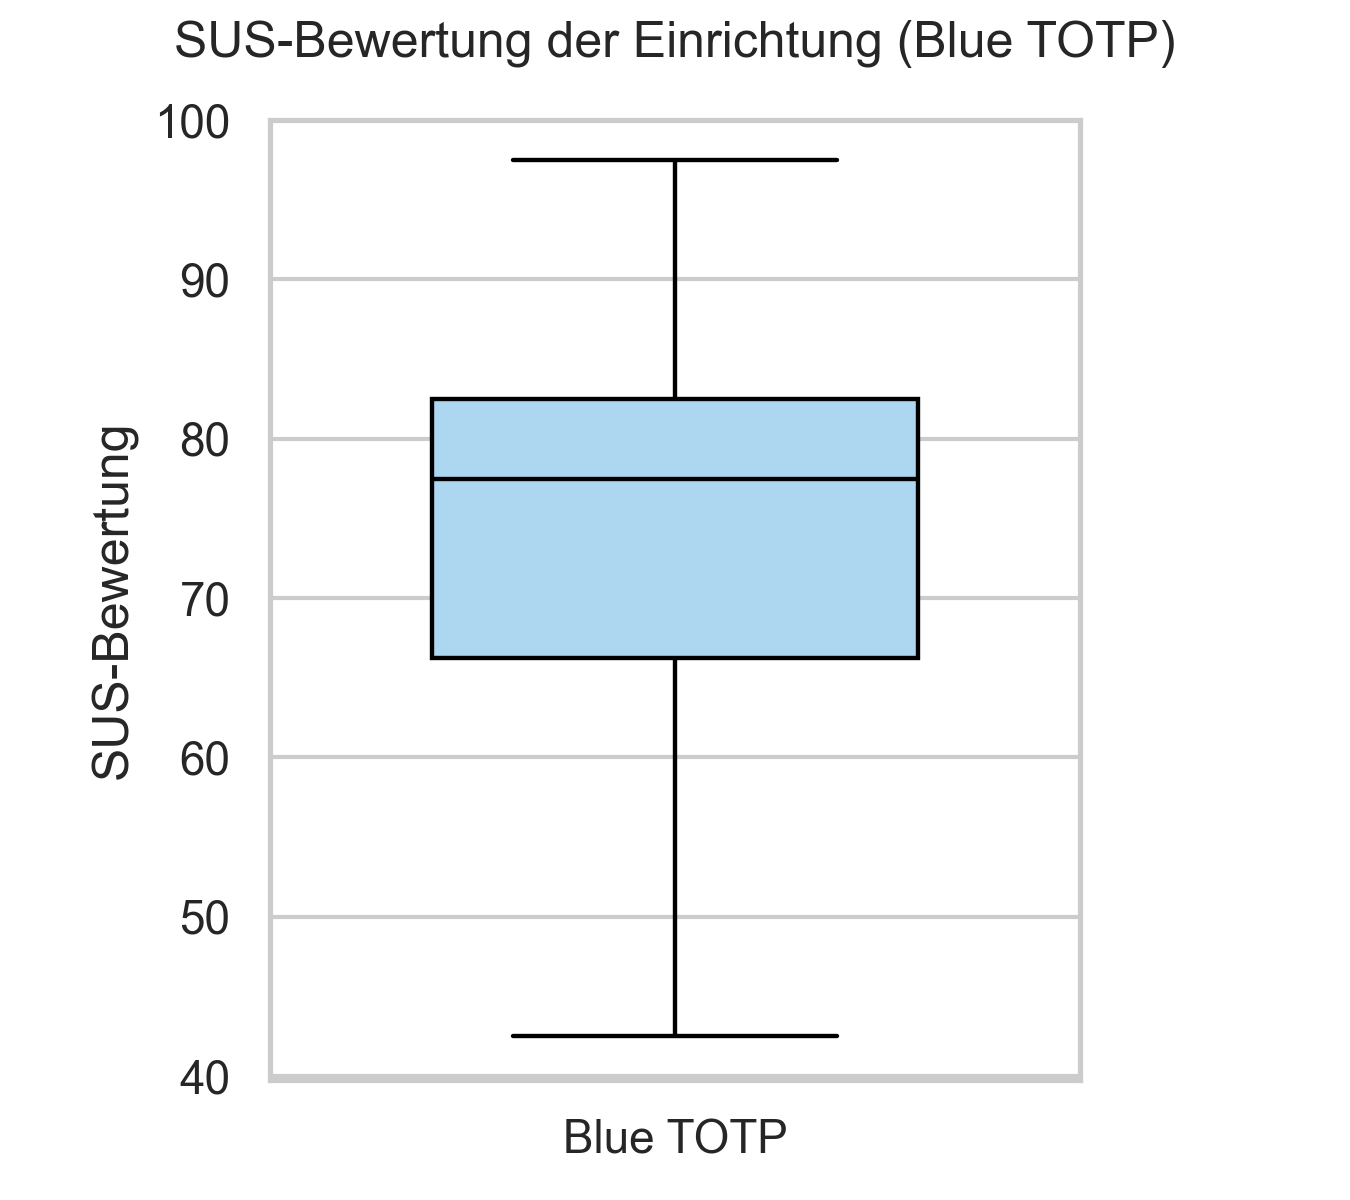
\includegraphics[width=.5\linewidth]{data_processing/questionaires/results/setup_sus_boxplot.png}
    \caption[SUS-Bewertung der Einrichtung von Blue TOTP]{SUS-Bewertung der Einrichtung von Blue TOTP}
    \label{fig: studie setup sus boxplot}
\end{figure}
Die schlechteste Bewertung erreichte ca. 43 Punkte, während die beste mit ca. 
98 Punkten nahe dem Maximum ist. Die Probanden haben die Einrichtung mit einem 
Median von 77.5 Punkten bewertet. Der Mittelwert liegt bei $75{,}8$ Punkten. 
Demnach liegt die Punktzahl über dem allgemeinen Vergleichswert von 68 Punkten.
\\\\
Zusätzlich wurde mit einer 7-stufigen Likert-Skala erfragt, wie nutzerfreundlich die Probanden das System insgesamt bewerten. Diese Werte werden mit einer zugehörigen SUS-Punktzahl gleichgesetzt \autocite{SUS11}. In Abb. \ref{fig: studie setup sus vs sus11} ist der Unterschied zwischen der empfundenen Nutzerfreundlichkeit und der eigentlichen SUS-Bewertung dargestellt.
\begin{figure}[h]
    \centering
    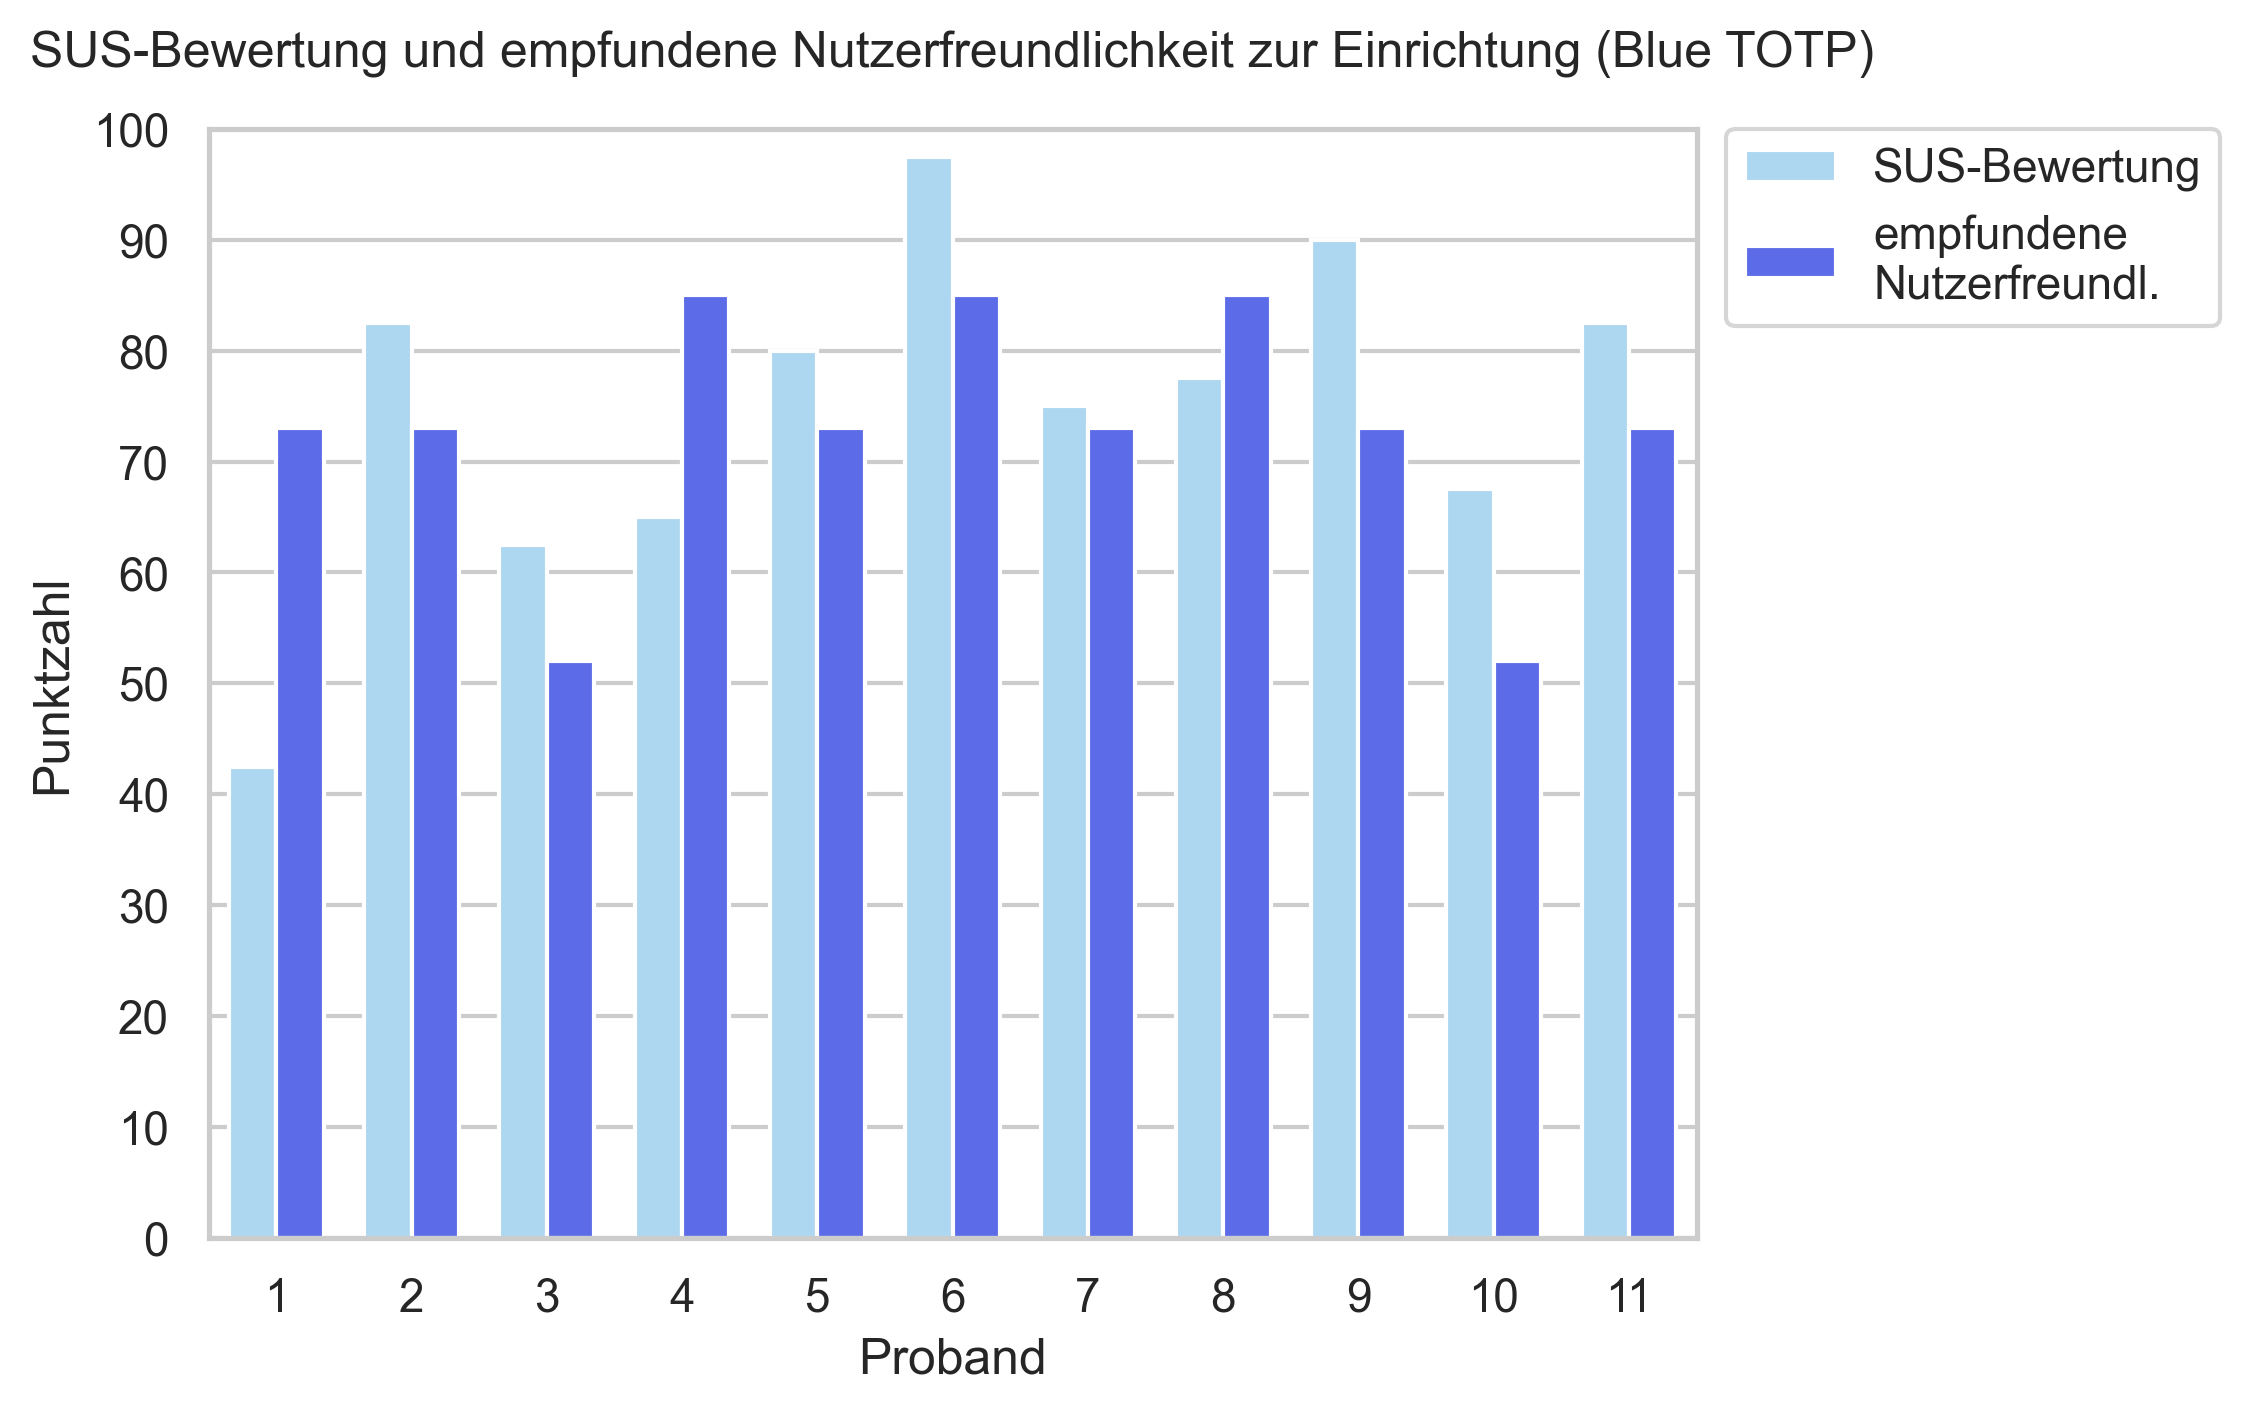
\includegraphics[width=.8\linewidth]{data_processing/questionaires/results/setup_sus_vs_sus11.png}
    \caption[SUS-Bewertung und empfundene Nutzerfreundlichkeit (Einrichtung Blue TOTP)]{SUS-Bewertung und empfundene Nutzerfreundlichkeit \autocite{SUS11} pro Proband zur Einrichtung von Blue TOTP}
    \label{fig: studie setup sus vs sus11}
\end{figure}
Die größte absolute Differenz hat Proband P1 mit ca. 30 Punkten, gefolgt von P4 
(20 Pkt.), P9 (17 Pkt.) und P10 (15 Pkt.). Die restlichen absoluten Differenzen 
schwanken zwischen 7 und 13 mit Ausnahme von P7 (2 Pkt.). Die 
Standardabweichung der absoluten Differenzen beträgt $7{,}7$ Punkte.
\\\\
\begin{table}[b]
    \centering
    \begin{center}
    \begin{tabular}{| l | c | c | c | c | c | c | c | c | c | c |}
        \hline
        \textbf{Aussage} & 1 & 2 & 3 & 4 & 5 & 6 & 7 & 8 & 9 & 10 \\
        \hline
        \textbf{Mittelwert} & $2{,}73$ & $3{,}18$ & $3{,}0$ & $2{,}82$ & $2{,}82$ & $3{,}27$ & $3{,}27$ & $3{,}27$ & $2{,}55$ & $3{,}0$ \\  
        \hline
    \end{tabular}
    \end{center}
    \caption[Durchschnittliche Bewertung pro Aussage des SUS (Einrichtung Blue TOTP)]{Durchschnittliche Bewertung pro Aussage des SUS (Einrichtung Blue TOTP)}
    \label{tab: studie setup sus mean per question}
\end{table}
Jeder Aussage im SUS-Fragebogen wird entsprechend der 5-stufigen Skala ein Wert 
von 0 bis 4 zugeordnet (0 sehr negativ behaftet, 2 neutral, 4 sehr positiv). 
Bildet man pro Aussage den Mittelwert über alle Probanden, erhält man die 
Ergebnisse in Tab. \ref{tab: studie setup sus mean per question}. Keine Aussage weist eine negativ behaftete Tendenz auf 
(kein Mittelwert kleiner 2). Den schlechtesten Durchschnitt bildet Aussage 9 
\glqq Ich habe mich bei der Nutzung des Systems sehr zuversichtlich gefühlt\grqq{} mit 
$\bar{x} = 2{,}55$. 
Besonders variieren die Werte bei Aussage 4 \glqq Ich glaube, ich würde die Hilfe 
einer technisch versierten Person benötigen, um das System benutzen zu können\grqq{}. 
Hier stimmten drei Probanden mit den Werten 1 oder 0 für die Richtigkeit der 
Aussage (also sie brauchen die Hilfe), während alle anderen mit den Werten 3 
oder 4 zum Ausdruck brachten, dass sie wenig bis keine Hilfe benötigen.